% $Id: template.tex 11 2007-04-03 22:25:53Z jpeltier $

\documentclass{vgtc}                          % final (conference style)
%\documentclass[review]{vgtc}                 % review
%\documentclass[widereview]{vgtc}             % wide-spaced review
%\documentclass[preprint]{vgtc}               % preprint
%\documentclass[electronic]{vgtc}             % electronic version

%% Uncomment one of the lines above depending on where your paper is
%% in the conference process. ``review'' and ``widereview'' are for review
%% submission, ``preprint'' is for pre-publication, and the final version
%% doesn't use a specific qualifier. Further, ``electronic'' includes
%% hyperreferences for more convenient online viewing.

%% Please use one of the ``review'' options in combination with the
%% assigned online id (see below) ONLY if your paper uses a double blind
%% review process. Some conferences, like IEEE Vis and InfoVis, have NOT
%% in the past.

%% Figures should be in CMYK or Grey scale format, otherwise, colour 
%% shifting may occur during the printing process.

%% These few lines make a distinction between latex and pdflatex calls and they
%% bring in essential packages for graphics and font handling.
%% Note that due to the \DeclareGraphicsExtensions{} call it is no longer necessary
%% to provide the the path and extension of a graphics file:
%% \includegraphics{diamondrule} is completely sufficient.
%%
\ifpdf%                                % if we use pdflatex
  \pdfoutput=1\relax                   % create PDFs from pdfLaTeX
  \pdfcompresslevel=9                  % PDF Compression
  \pdfoptionpdfminorversion=7          % create PDF 1.7
  \ExecuteOptions{pdftex}
  \usepackage{graphicx}                % allow us to embed graphics files
  \DeclareGraphicsExtensions{.pdf,.png,.jpg,.jpeg} % for pdflatex we expect .pdf, .png, or .jpg files
\else%                                 % else we use pure latex
  \ExecuteOptions{dvips}
  \usepackage{graphicx}                % allow us to embed graphics files
  \DeclareGraphicsExtensions{.eps}     % for pure latex we expect eps files
\fi%

%% it is recomended to use ``\cite{sec:bla}'' instead of ``Fig.~\ref{sec:bla}''
\graphicspath{{figures/}{pictures/}{images/}{./}} % where to search for the images

\usepackage{microtype}                 % use micro-typography (slightly more compact, better to read)
\PassOptionsToPackage{warn}{textcomp}  % to address font issues with \textrightarrow
\usepackage{textcomp}                  % use better special symbols
\usepackage{mathptmx}                  % use matching math font
\usepackage{times}                     % we use Times as the main font
\renewcommand*\ttdefault{txtt}         % a nicer typewriter font
\usepackage{cite}                      % needed to automatically sort the references
\usepackage{tabu}                      % only used for the table example
\usepackage{booktabs}                  % only used for the table example
%% We encourage the use of mathptmx for consistent usage of times font
%% throughout the proceedings. However, if you encounter conflicts
%% with other math-related packages, you may want to disable it.


%% If you are submitting a paper to a conference for review with a double
%% blind reviewing process, please replace the value ``0'' below with your
%% OnlineID. Otherwise, you may safely leave it at ``0''.
\onlineid{0}

%% declare the category of your paper, only shown in review mode
\vgtccategory{Research}

%% allow for this line if you want the electronic option to work properly
\vgtcinsertpkg

%% In preprint mode you may define your own headline.
%\preprinttext{To appear in an IEEE VGTC sponsored conference.}

%% Paper title.

\title{Generating alphabets: a medium-independent framework for the creation of systems of symbols.}

%% This is how authors are specified in the conference style

%% Author and Affiliation (single author).
%%\author{Roy G. Biv\thanks{e-mail: roy.g.biv@aol.com}}
%%\affiliation{\scriptsize Allied Widgets Research}

%% Author and Affiliation (multiple authors with single affiliations).
%%\author{Roy G. Biv\thanks{e-mail: roy.g.biv@aol.com} %
%%\and Ed Grimley\thanks{e-mail:ed.grimley@aol.com} %
%%\and Martha Stewart\thanks{e-mail:martha.stewart@marthastewart.com}}
%%\affiliation{\scriptsize Martha Stewart Enterprises \\ Microsoft Research}

%% Author and Affiliation (multiple authors with multiple affiliations)
\author{Serhii Hamotskyi\thanks{e-mail: shamotskyi@gmail.com}\\ %
        \scriptsize National Technical University of Ukraine "Igor Sikorsky Kyiv Polytechnic Institute"\\
\and Sergii Stirenko\\
        \thanks{sergii.stirenko@gmail.com}
        \scriptsize National Technical University of Ukraine "Igor Sikorsky Kyiv Polytechnic Institute"\\
\and Yuri Gordienko\\
        \thanks{yuri.gordienko@gmail.com}
        \scriptsize National Technical University of Ukraine "Igor Sikorsky Kyiv Polytechnic Institute"}

%% A teaser figure can be included as follows, but is not recommended since
%% the space is now taken up by a full width abstract.
%\teaser{
%  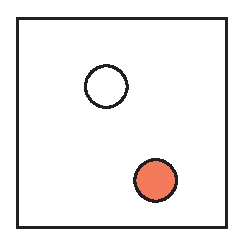
\includegraphics[width=1.5in]{sample.eps}
%  \caption{Lookit! Lookit!}
%}

%% Abstract section.
\abstract{In this paper, we discuss the generation of symbols (and alphabets) based on specific user requirements (medium, priorities, type of information that needs to be conveyed). A framework for the generation of alphabets is proposed, and its use for the generation of a shorthand writing system is explored. We discuss the possible use of machine learning and genetic algorithms to gather inputs for generation of such alphabets and for optimization of already generated ones. The alphabets generated using such methods may be used in very different fields, from the creation of synthetic languages and constructed scripts to the creation of sensible commands for Human-Computer Interfaces, such as mouse gestures, touchpads and eye-tracking cameras.
} % end of abstract

%% ACM Computing Classification System (CCS). 
%% See <http://www.acm.org/class/1998/> for details.
%% The ``\CCScat'' command takes four arguments.

\CCScatlist{ 
  \CCScat{H.5.2}{Information interfaces and presentation}%
{User Interfaces}{Ergonomics}; %%TODO
}

%% Copyright space is enabled by default as required by guidelines.
%% It is disabled by the 'review' option or via the following command:
% \nocopyrightspace

%%%%%%%%%%%%%%%%%%%%%%%%%%%%%%%%%%%%%%%%%%%%%%%%%%%%%%%%%%%%%%%%
%%%%%%%%%%%%%%%%%%%%%% START OF THE PAPER %%%%%%%%%%%%%%%%%%%%%%
%%%%%%%%%%%%%%%%%%%%%%%%%%%%%%%%%%%%%%%%%%%%%%%%%%%%%%%%%%%%%%%%%

\begin{document}

%% The ``\maketitle'' command must be the first command after the
%% ``\begin{document}'' command. It prepares and prints the title block.

%% the only exception to this rule is the \firstsection command
\firstsection{Introduction}

\maketitle

%% \section{Introduction} %for journal use above \firstsection{..} instead

The need to create writing systems has been with humankind since the dawn of time, and they always evolved based on the concrete challenges the writers faced. For example, the angular shapes of the runes are very convenient to be carved in wood or stone~\cite{williams1996origin}. Alphabets have been created for various purposes, each subject to its own constraints (morse code, shorthand writing, etc.). The rapid increase of available mediums in the recent decades determined the need for many more alphabets, for very different use cases, such as controlling computers using touchpads, mouse gestures or eye tracking cameras. 

We started researching this topic by attempting to manually create a system for writing in shorthand (extremely simplified writing used in courtrooms or journalism optimized for writing speed, not readability), since we were not satisfied by existing ones, and then attempting to automate the process. There have been extremely few noteworthy developments in shorthand since the creation of Teeline Shorthand in 1968, and there have been no attempts known to us of using genetic algorithms or any form of automated generation for their creation.

 Many approaches for the generation of alphabets have been used, but we are not familiar with a formalized system for their generation. Manually generated alphabets are usually suboptimal. For example, it might be argued that the Latin alphabet favours the writer more than the reader, since it evolved under the constraints of pen and paper, and those constraints are much less relevant in the computer age; readable symbols could be created using much less space. Fonts which try to overcome this limitation exist, for example using dots in the place of strokes.~\cite{dotsies}. In a similar fashion, many systems do not use the possibilities given by the medium or context (for example multi-touch gestures). A formalized framework or software application capable of gathering requirements, generating symbols, grading them on a set of criteria and mapping them to meanings may be able to overcome many of those limitations.

In this paper, the authors discuss metrics for a rational alphabet of symbols, basing themselves on their experience of creating the shorthand system, and suggest a framework for the rational generation of alphabets. The application of the suggested requirements to the creation of a shorthand system is shown as example. The analysis of data that is to be conveyed, the generation of symbols, their grading according to certain criteria and the analysis of resulting alphabets is discussed.

The proposed framework is formulated so as to be used independently of the medium; that is, the generation of requirements, the rating of the generated glyphs, their mapping to meanings and the evaluation of the final alphabet should be applicable to any medium --- be it a touchpad, an eye-tracking camera, a shorthand system, or 3D gestures with an additional fourth dimension added by pressing a button.

\section{High-level overview}

The basic framework as proposed consists of five steps, outlined in Fig. 1. For the purposes of this paper, "glyph" is defined as unique mark/symbol in a given medium; 2D symbols without varying width are used in this paper as examples. "Symbol" is defined as a glyph with a meaning attached to it. "Alphabet" is defined as a system of such symbols, including possible modifiers and conventions.

In the proposed framework, glyphs are generated and rated first, and meanings are assigned later; only then the alphabet as a whole is rated. This two-step process design choice is based on performance reasons (mutating individual glyphs and their meanings at the same time is too complex for any reasonably-sized alphabet) and is meant as a starting point for further research and adaptation. 

\begin{figure}[tb]
\centering
        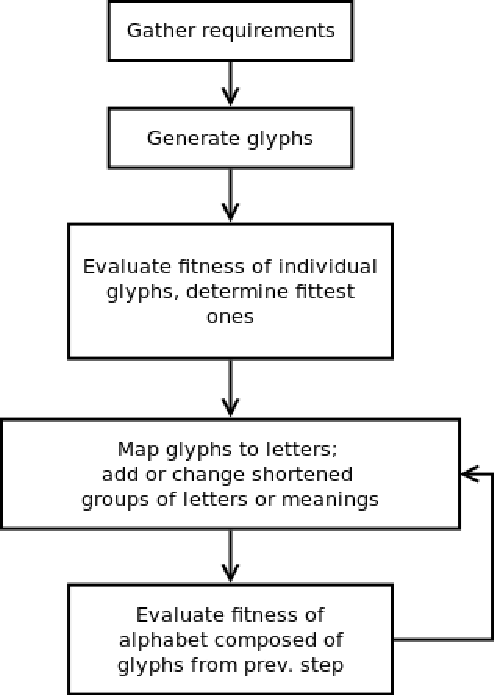
\includegraphics[width=0.75\hsize]{f.pdf}
\caption{Basic description of framework.}
\end{figure}

\section{Characteristics of a rational alphabet}

%% As this is a framework for the creation of alphabets in general, the goal is not to give any final recommendations about concrete alphabets, as they should be formulated individually for each alphabet.


The following desirable characteristics (and possible metrics) should generalize well for almost any alphabet, independently from the medium, dimensionality, and purpose. The vocabulary related to writing 2D characters with a pen or stylus is used, but this can be replaced with any other device.  

Most of these characteristics are intimately interconnected.


\subsection{Writing comfort and ergonomics}
If such a system is to be used often, writing comfort becomes a main concern, and might mean the difference between the system being used or not used at all. 
("The best camera is the one that's with you" goes the photography adage.) %qq
For our purposes, we define comfort as "how easy and enjoyable is to use the alphabet". This might depend on the following factors:
\begin{itemize}
        \item How much mental effort does the recall of the symbols require (ease of recall)
                \begin{itemize}
                        \item How familiar are the symbols to the user at the moment he is writing. 
                                \begin{itemize}
                                        \item Similarity to already known stimuli
                                        \item Availability of a mnemonic system
                                \end{itemize}
%%                        \item how much mental effort does the emph{creation} of the symbols require (in case the glyph is composite).
                \end{itemize}
        \item Fluency/flow, not meant as relationship between person and alphabet, but as characteristic of the alphabet itself. Both for individual letters and their usual combinations.
        \item Physical limitations. For example, some strokes might be easier to write if someone is right-handed, or holds his pen in a certain way.
\end{itemize}


Quantifying the above is non-trivial.  Additionally, the subjective reactions to glyph might vary between people, differences due to age, cultural and/or language background are probable. This might be a promising area to study with the help of machine learning. Data like "Symbols similar to X perform poorly with demographic Y" would be valuable for creating alphabets when something about the probable users is known (which alphabet or writing system is more familiar to them? How much new information are they probably able to learn and for how much they are able to retain it? Did they learn thousands of hieroglyphics since they were children? How motivated are they?). 

We suggest the following metrics as starting points for future research and discussion:

\subsubsection{Mental effort}
We think that this would be best measured via existing methods. Changes in pupil size might be an especially interesting avenue in this aspect~\cite{Alns2014PupilSS}, as something objective and easy to measure.

If memory is more an issue than cognitive load, than generating the alphabet in such a way so that creating a mnemonic system for it is possible might be a way to decrease mental effort. As a very trivial example of this, when we were manually creating our shorthand system, we decided to encode 
 time, modality, and person via a single glyph consisting of three parts, which allowed to considerably shorten groups like "they would have been able to" (\autoref{i:sample}). Memorizing all the possible combinations would be nonsensical, but generating the glyph again mentally from its parts as it's written is easier. 

\begin{figure}
\centering
        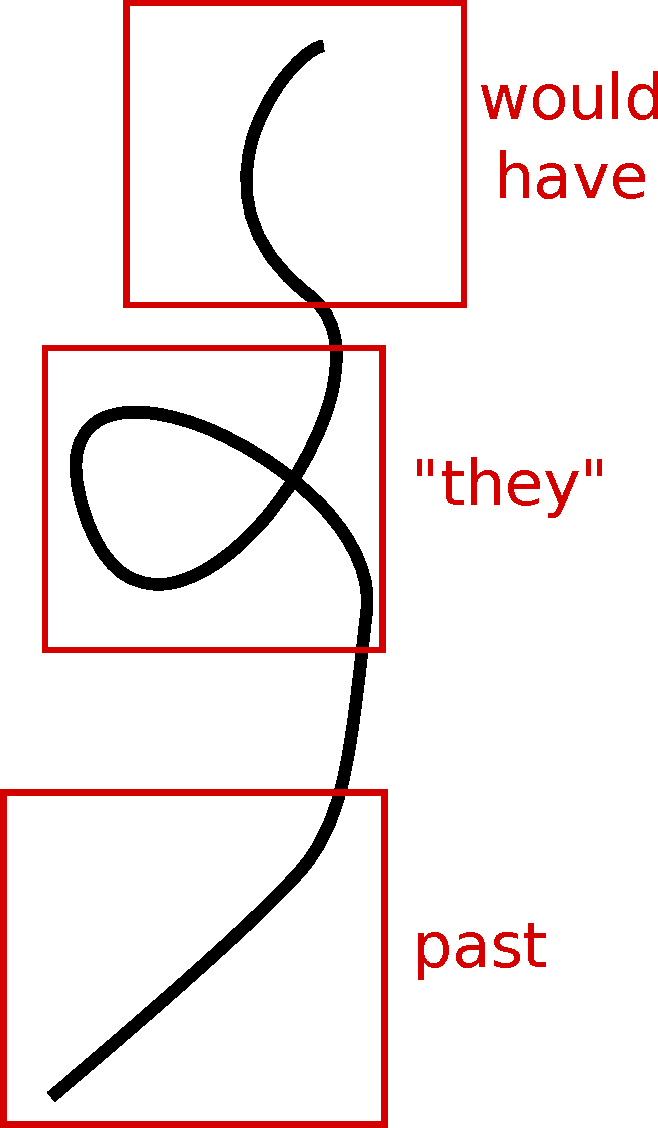
\includegraphics[width=0.35\hsize]{woudl.pdf}
        \caption{Example of composite glyph that doesn't need to be memorized in full}
        \label{i:sample}
\end{figure}

\subsubsection{Fluency}
Possible metrics for fluency could be:
\begin{itemize}
        \item Number of shap angles per glyph.
        \item Curvature per glyph. Both can be defined as sum the sum of absolute changes in direction per unit of distance. For example, if we represent a glyph as a polygonal path, of \(n\) lines, we can quantify this as
                \(c=\sum_{i=1}^n|L_n(j_i, j_{i+1})|\), where \(n\) is the number of  points used to approximate the curve, \(L\) is the angle between two adjacent lines  \(j_i, j_{i+1}\).
        \item Ratio of strokes that mean something semantically, as opposed to "connecting one glyph with another", to the entire number.
        \item Number of easily connectable glyphs following each other in an average text, so that as little unnecessary movements are made. For example, given a representative source text, 
                \[c=\sum_{i=1}^n\sum_{j=1}^nE(g_i, g_j)P(g_i,g_j)\], where \(n\) is the number of existing glyphs, \(E(g_i, g_j)\) is how "easy" are the two glyph to connect, \(P(g_i, g_j)\) is how the probability \(g_i\) will be directly before \(g_j\).
\end{itemize}


\subsection{Writing speed}
Defined not as "how fast the pen moves", but rather "how much time is needed to convey the needed information".

\begin{itemize}
        \item How fast are individual glyphs to write. This intersects heavily with "Fluency".
                \begin{itemize}
                        \item Fluency from the subsection above.
                        \item How much the pen needs to travel to form the glyph; glyph "length".
                \end{itemize}
        \item How much "meaning" can be encoded in one glyph. This is directly related to redundancy and entropy, discussed in the following sections.
        \item The more simple glyphs should be mapped to the most common symbols.
\end{itemize}

Glyph length could be measured by converting it to a Bezier curve and calculating its length. When defined in connection to the meaning conveyed (rate), real-life experiments would be needed. 

A potentially interesting experiment would be timing people using the system, and dividing the amount of information written by the time taken; but this would raise questions about the input information. Accurately calculating the entropy of the conveyed information for this purpose would be practical only for alphabets used in very narrow and formalized contexts.

\subsection{Ease of recognition}

Intimately related to the previous subsection.

\begin{itemize} 
        \item How different are the glyphs between each other
        \item how much are distortions likely to worsen the recognition of the glyphs.
\end{itemize}

Additionally,  here various memory biases and characteristics of human memory will be at play (see, for example,the Von Restorff effect~\cite{hunt1995subtlety}).

\subsection{Universality}

Ideally, the glyphs should generalize well. That means that once learned for styluses,the same alphabet shouldn't be too hard to port to other mediums without losing many of the above mentioned characteristics. Additionally, learning to use it should be relatively painless. Not needed in all contexts, but mostly it's a desirable characteristic. Excepting changes of dimensionality (3D-gestures might be hard to port to a 2D-stylus), this is probably the hardest to quantify and account
for.

\section{Gathering requirements for the needed alphabet}

As mentioned in the Introduction, most writing systems have been heavily influenced by the constraints inherent in their area of use --- purpose, characteristics of the information they needed to convey, materials used. When synthetic systems of symbols are created or generated, they similarly are constrained, but can't be polished by millennia of continuous use. And lastly, even if there were millennia to let those systems evolve, even naturally evolving systems tend to converge towards local optima rather than a global optimum (as is the case with genetic algorithms). Requirements and use patterns may gradually change, while the systems may be stuck in a state that is not optimal anymore, being unable to sacrifice short-term fitness for long-term fitness. (This might be considered an example of path dependence.) Therefore, before attempting to create a system from zero, a very careful analysis of the requirements and limitations is needed.

Above, we mentioned general characteristics and metrics. For our example of creating a shorthand system (trivial use case), on a more practical note, the balance between the following may be considered:
\begin{enumerate}
        \item On a purely symbolic level:
        \begin{enumerate}
                \item Writing letters
                \begin{enumerate}
                        \item number of strokes needed to encode individual letters
                        \item complexity of the resulting glyph
                        \item similarity of each glyph to it's English alphabet counterpart, if there is one.
                \end{enumerate}
                \item Writing words
                \begin{enumerate}
                        \item connections between individual letters (glyphs)
                        \item how likely are letters that are easy to connect to each to be represented by easily connectable glyphs
                        \item if all existing glyphs are not identical in complexity, what is the ratio of easy-to-write glyphs to the complex ones in a typical text (the bigger the ratio, the better)
                \end{enumerate}
        \item Writing sentences: are there any often-repeating words or groups of words which, when replaced by a shorter, even if complex, symbol, would lead to a gain in time? ("The" as a typical example).
        \end{enumerate}
        \item On a semantic level: Are there any grammatical categories or modalities that are represented in natural text with many letters, that when replaced by a single glyph or a modifier, would lead to a gain in time? (tenses, number, gender, hypotheticals, ...). The encoding of person, time and modality mentioned above, if one is to be used, would happen at this abstraction level.:w
        \item On an information theoretical level: How much redundancy is needed? How many errors in transcription can happen before the message becomes either unreadable or its meaning is distorted?  (Natural languages  are redundant via multiple mechanisms, notably via agreement in person, gender, case...~\cite{bussmann2006routledge} Errors or interferences will still allow to understand what’s being said, up to a certain point. This may not be the case for constructed writing systems, if they are built with low redundancy)~\cite{reza1961introduction}.
\end{enumerate}

As for quantifying the above, a basic way to do this four our shorthand example would be analyzing source texts by the person (or representative sample of people) who will be using the system, to fit it to their speech patterns and word use. At the end, the following very basic information should be available:

\begin{itemize}
        \item frequencies of individual letters \(p_i\)
        \item most-needed connections \(c_{ij}\)
\end{itemize}

Each of the generated glyphs can have three possible starting and ending strokes, represented by integers, and positioned at different heights.\(I_s, I_e=\{0, 1, 2\}\) Glyphs \(i, j\) where \(i_e=j_s\) are considered easily connectable. Using this information, later we can map the glyphs to meanings in such a way, that the letters that are most likely to follow each other are more likely to be
represented by easily connectable glyphs. The problem would be trivially solvable by having all glyphs start and end at the same point, but this would make it harder to differentiate the individual glyphs.

\section{Generation of the glyphs}
The second part of the proposed framework is the generation of possible glyphs. In this paper, Bezier curves have been used to generate the glyphs and calculate some of the needed metrics.
During the generation of the example glyphs, we made the following assumptions about the alphabet for which the glyphs are generated:
\begin{enumerate}
        \item The glyphs have a definite starting and ending point; the number of such points is limited, to facilitate connecting the symbols to each other.
        \item The stroke width does not vary (as, for example, in the case of Pitman shorthand), because of the low availability of pens able to convey even two levels of thickness and of low average penmanship skill in most people. (Though using it as a third or fourth dimension would certainly be possible.)
        \item The symbols will fit into a square bounding box.
\end{enumerate}

For each letter, multiple glyphs are generated. The generation of glyphs starts by fixing a definite starting and ending point and then adding a semi-random number of control points. The number of control points used in the generation of the specific glyph is selected via a normal distribution, with the average number being the mean of the distribution and with standard deviation being calculated based on the maximum number of control points. While one of the criteria for the glyphs is their
simplicity, extremely simple symbols are counterproductive, and we needed to prevent the alphabet from degenerating to straight and diagonal lines. Additionally, variation in the gene pool is crucial in genetic algorithms, if one is to be used later on. Therefore, a degree of randomness in all phases is needed, and this is one way to provide it. Figures 2-5 are examples of glyphs generated using the above rules.

\begin{figure}[tbp]
\centering
        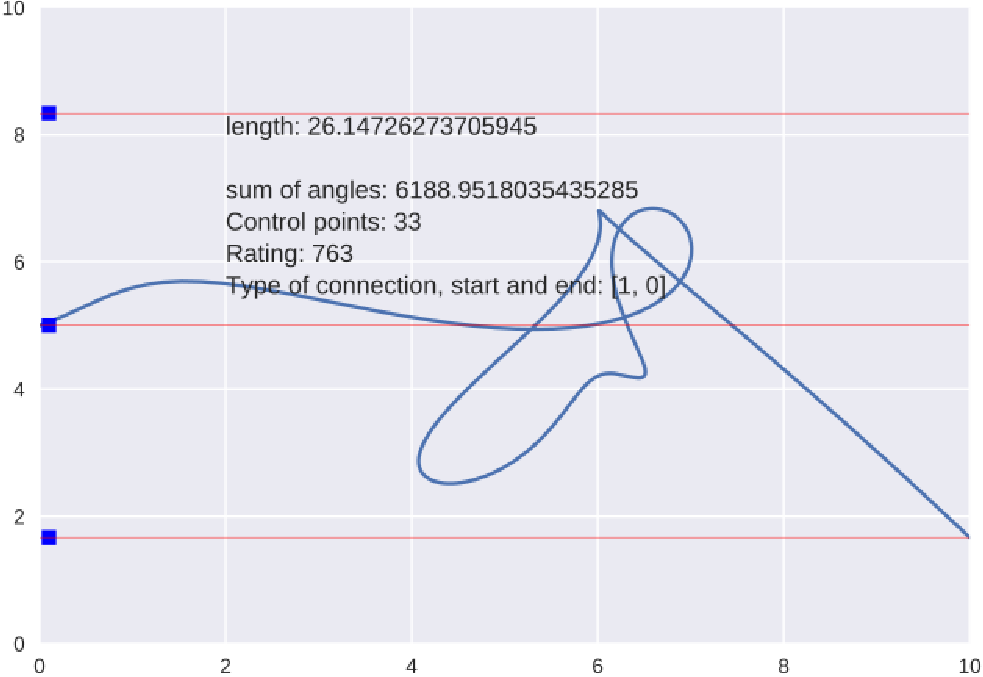
\includegraphics[width=0.75\hsize]{e1.pdf}
\caption{Example of generated glyph with low fitness}
\end{figure}
\begin{figure}[tbp]
\centering
        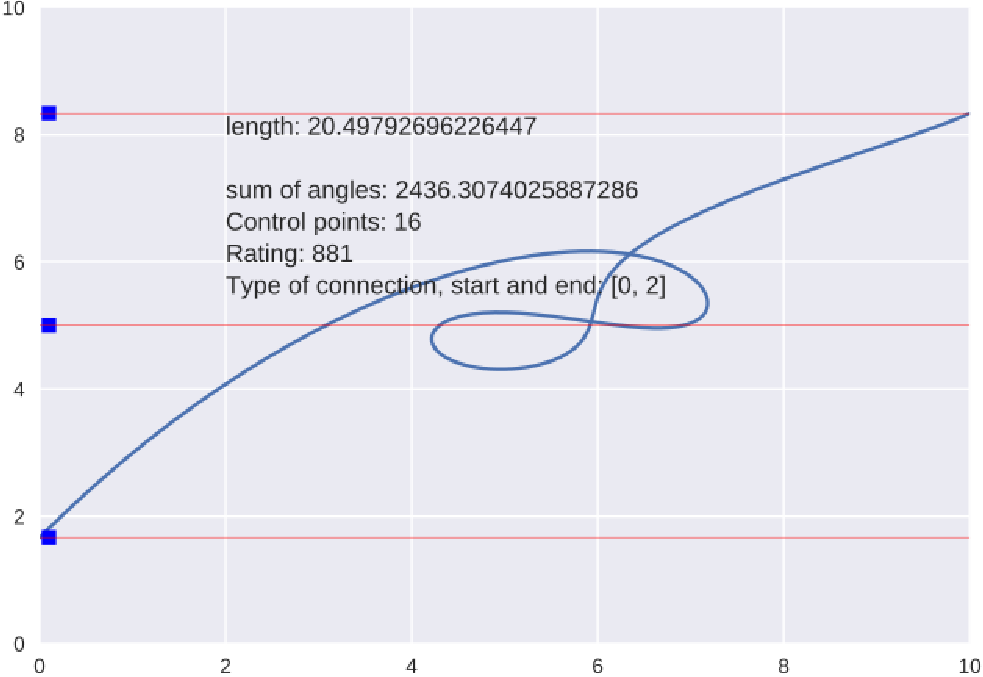
\includegraphics[width=0.75\hsize]{e3.pdf}
\caption{Glyph with higher fitness      }
\end{figure}
\begin{figure}[tbp]
\centering
        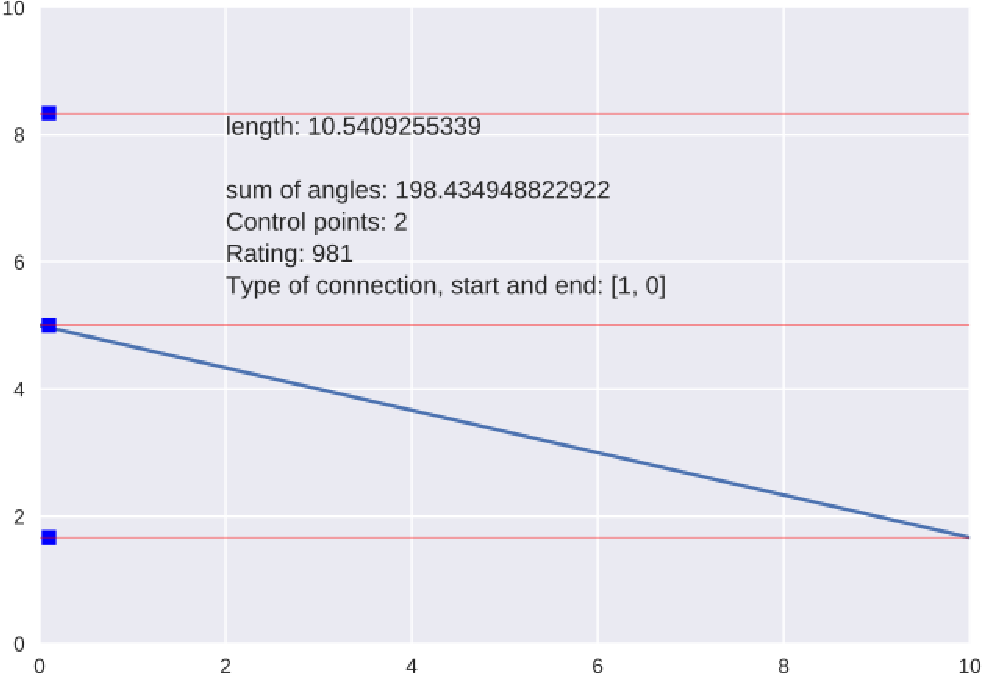
\includegraphics[width=0.75\hsize]{e4.pdf}
\caption{Too many extremely simple symbols would not be desirable}
\end{figure}
\begin{figure}[tbp]
\centering
        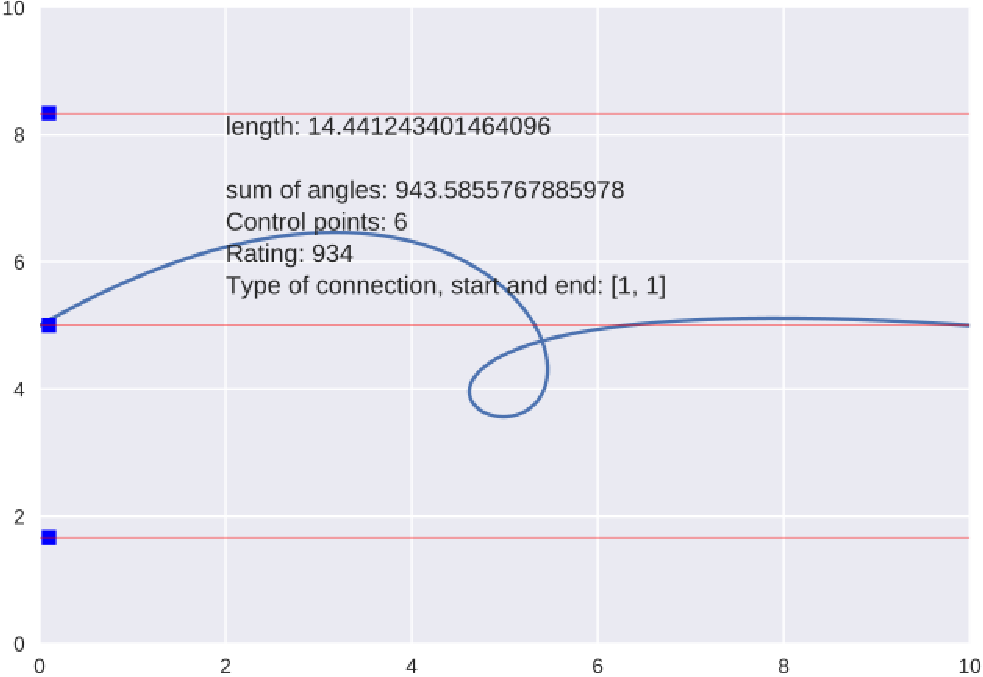
\includegraphics[width=0.75\hsize]{e2.pdf}
\caption{The simpler a glyph is, the higher fitness it has}
\end{figure}

\section{Evaluating the fitness of the individual glyphs}
In this stage, the fitness of each glyph is determined. Many approaches are possible, and they heavily depend on the context and the medium for which the generation is being done. For our shorthand system, the main criteria were length and simplicity. The number of control points has been used as a proxy of fitness and has been partly accounted for in the generation phase (empirically, the more control points the more chaotic the glyph is). The second metric was flow. For our purposes,
flow was defined as \(\frac{c}{l}\), where \(c\) is the sum of the angles in the polygonal representation of the curve (informally, how curved the glyph is; the more curves there are and the sharper the individual curves are, the bigger the value is), and \(l\) is the length of the curve (a certain amount of curves on a large glyph should not be penalized as much as the same amount on a smaller one). C is calculated by converting the curve between the first adjoining control points to a polygon, summing the absolute value of the angles between all adjoining lines, and repeating the process for all the successive control points.
\(c=\sum_{i=1}^n\sum_{j=2}^{p}L_n(j_i, j_i-1)\), where \(n\) is the number of control points,  \(p\) is the number of lines used to approximate the curve, L is the angle between two lines,  and \(j_i\) is the line after the control point \(i\). 

The reasons for defining \(c\) as we did are manifold, one of them being that a very similar metric is used for evaluating the similarity of the two glyphs to each other. Much better metrics are possible.


Additionally, machine learning would open the doors for custom-tailored systems, where users rate some symbols and based on their feedback predictions are made about what other symbols they might like, remember and use. And, as mentioned previously, their particular use patterns might dictate different mappings of symbols to meanings (letters, actions, preferences). 
\section{Mapping symbols to meanings}
The first mapping of the generated glyphs, before its fitness is rated, is necessarily very tentative. At the beginning, we suggest just mapping the letters to glyphs by ordering the glyphs in decreasing order of fitness and pairing them with letters, ordered by their frequency. This would give a good starting point, which can be further improved in the next step by taking into account how easy the letters are to connect and the other requirements. 

In this paper we have not touched grammatical modalities and ways to shorten them in great detail, as they would merit quite a lot more research and space (and, probably, their own paper); regardless, they would have their place at this step of the framework. 
\section{Evaluating the fitness of an alphabet}
Four our shorthand, we have limited ourselves to the following three basic criteria:
%qq criteria/characteristics/requirements
\begin{enumerate}
        \item As much high-fitness glyphs as possible
        \item Letters which are found the most often should be represented by the glyphs of the highest fitness (that is, be as simple as possible).
        \item The letters should be unlike to each other
\end{enumerate}

The most important requirement is for the letters to be unlike each other. This is needed both for the resulting text to be readable (the existance of a 1-to-1 mapping between a text written in shorthand and a normal text, or at least for the resulting text being readable using contextual clues) and for improving the memorization of the glyphs (memorizing many similar stimuli is much harder than many different ones, unless a good framework for memorization is given, such as dividing symbols in parts). 

For our purposes histogram comparison was the most straight-forward to implement. The data for the histogram is provided by the angles computed at the previous step. Basic shapes and turns would be recognizable, and the difference between the two makeshift histograms would approximate the difference between the glyphs. Here, \(D_{ij}\) is the difference between glyphs \(i, j\).

Therefore, one formula for the fitness could be:
\[
f=\sum^{n}_{i=1}f_i+
\sum^{n}_{i=1}\sum^{n}_{i=1}D_{ij}+
\sum^{n}_{i=1}f_ip_i
\]
and the glyphs are picked so that the above formula is maximized. (The formula above does not include connections.)

A genetic algorithm at this point would attempt adding/removing/moving control points, switching glyphs between letters, introducing mirror-distortions etc. etc.

\section{Discussion and future work}
The basic ideas of this framework can be applied for the generation of any alphabet used in the real world. For touchpads, for example, connections may be built not using three possible endings, but 2D-points on the screen instead, and multitouch and weight-sensitivity may be included in the generation. By adding dimensions, 3D-gestures alphabets may be created. Much better heuristics for fitness may be created by more precise algorithms, machine learning and use of biology and cognitive science. 

The approaches demonstrated here are general enough to allow an enormous amount of flexibility in the kind of alphabets they may be used to create.

One of the more interesting avenues of further research would be creating algorithms for mapping glyphs to semantics, both to letters and to more complex grammar categories or structures. 

\section{Conclusion}
In this work in progress paper, the question of generating alphabets for various purposes and mediums is discussed. Basic requirements are formulated, along with possible metrics and avenues of further research. A framework for the generation of alphabets is formulated. Elements of the proposed framework are demonstrated using the generation of symbols for a shorthand writing system. The use of source data (both source texts and experimental data) for the creation of alphabets fitting a
certain context and the use of machine learning to build better fitness heuristics and to predict the potential fitness of glyphs is discussed. The approach shown may be used to generate alphabets for a very wide variety of methods and purposes.


%% if specified like this the section will be committed in review mode
%\bibliographystyle{abbrv}
\bibliographystyle{abbrv-doi}
%\bibliographystyle{abbrv-doi-narrow}
%\bibliographystyle{abbrv-doi-hyperref}
%\bibliographystyle{abbrv-doi-hyperref-narrow}

\bibliography{mybib}
\end{document}
